% !TEX TS-program = lualatex
% !TEX encoding = UTF-8

% This is a simple template for a LuaLaTeX document using gregorio scores.

\documentclass[letterpaper,12pt]{book} % use larger type; default would be 10pt

\input{header.inc}

\geometry{letterpaper,outer=0.4in,inner=0.9in,top=0.6in,bottom=0.8in}

\begin{document}

\printsmalltitle{Beate Pastor Petre}

\garamondbig
\greannotation{Hymn.}
\greannotation{4.}
\gregorioscore{241_hy--beate_pastor_petre--solesmes}

\begin{centering}

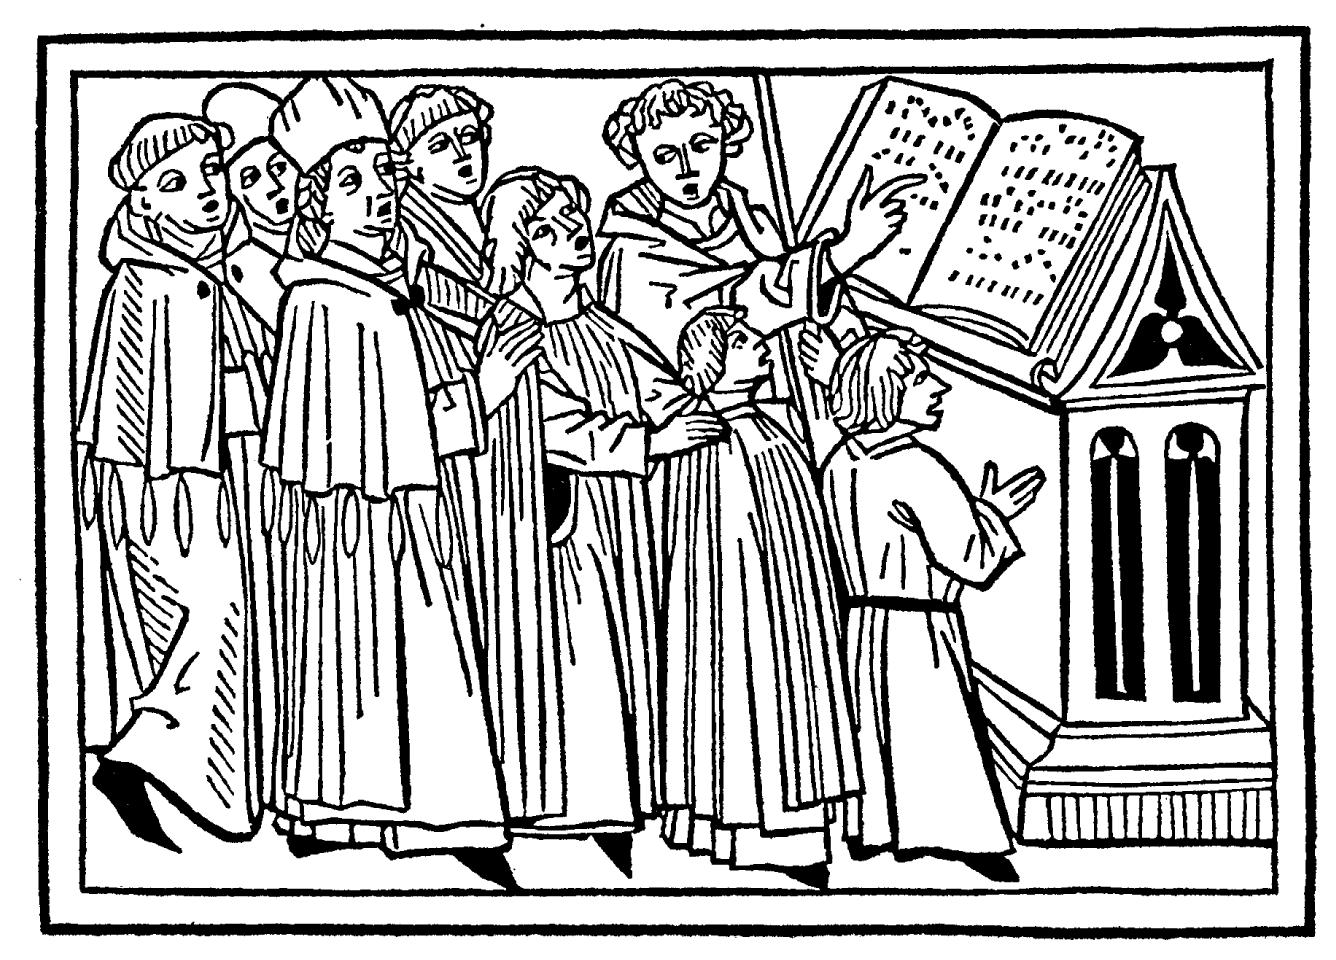
\includegraphics[width=0.55\textwidth]{../242_clipart.jpg}

\end{centering}

\vfill
\pagebreak

\printsmalltitle{Prayer for the Pope}

\printsmalltitle{Oremus Pro Pontifice}

\greannotation{1.}
\gregorioscore{243_va--oremus_pro_pontifice--solesmes}

\bigskip

\Vbar{}.~Tu es Petrus.

\Rbar{}.~Et super hanc petram ædificábo Ecclésiam meam.




\end{document}